
\begin{questions}
\question{
Play with the exchange-correlation function
}
\begin{solution}
For the density we have two different cases, when the spins are parallel and when they are antiparallel. When they are antiparallel the density looks like
\begin{equation}
  n_{\uparrow \downarrow} (\vec{r},\vec{r}') = \sum_{k_i}\sum_{k_j} \frac{1}{V^2} = \frac{(N/2)(N/2)}{V^2} = n_\uparrow n_\downarrow.
\end{equation}
And the corresponding pair-correlation function is then
\begin{equation}
  g_{\uparrow \downarrow} (\vec{r},\vec{r}')  = \frac{n_{\uparrow \downarrow} (\vec{r},\vec{r}')}{n_\uparrow n_\downarrow} = 1.
\end{equation}
When the spins are parallel is not trivial
\begin{equation}
  n_{\uparrow \uparrow}(\vec{r},\vec{r}') = \sum_{k_i} \sum_{k_j\neq k_i} \left( \frac{1}{V^2} - \frac{1}{V^2}e^{i(\vec{k}_i - \vec{k}_j)\cdot(\vec{r}- \vec{r}')} \right).
\end{equation}
Once again we now how to transform sums to integrals
\begin{equation}
  \sum_{\vec{k}} \longrightarrow \frac{V}{(2\pi)^3} \int d\vec{k},
\end{equation}
using this we transform this equation into
\begin{equation}
  n_{\uparrow \uparrow}(\vec{r},\vec{r}') = n_{\uparrow \uparrow} - \int_{|\vec{k}|<k_F} \frac{d \vec{k}}{(2\pi)^2} \int_{|\vec{k'}|<k_F} \frac{d \vec{k}'}{(2\pi)^3} e^{i(\vec{k}_i - \vec{k}_j)\cdot(\vec{r}- \vec{r}')} .
\end{equation}
We can propose a similar change of variable as in the last section for the distance $\delta = |\vec{r} - \vec{r}'|$, and the result after integrating will be
\begin{equation}
  g_{\uparrow \uparrow}(\vec{r},\vec{r}') = \frac{n_{\uparrow \uparrow}(\vec{r},\vec{r}')}{n_{\uparrow \uparrow}} = 1 - \left( \frac{3\sin(k_F\delta) - 3(k_F\delta)\cos(k_F\delta)}{(k_F\delta)^3} \right)^2.
\end{equation}
Hence the total exchange correlation function is
\begin{equation}
  g(\vec{r},\vec{r}')  = 2 - \left( \frac{3\sin(k_F\delta) - 3(k_F\delta)\cos(k_F\delta)}{(k_F\delta)^3} \right)^2.
\end{equation}
Finally, the pair density is
\begin{equation}
  \begin{aligned}[b]
    n(\delta) &= \frac{n}{2}\left( 2 - \left( \frac{3\sin(k_F\delta) - 3(k_F\delta)\cos(k_F\delta)}{(k_F\delta)^3} \right)^2\right). \quad_\blacksquare
  \end{aligned}
\end{equation}

 We can see this function ploted on fig. \ref{fig:hole}

 \begin{center}
   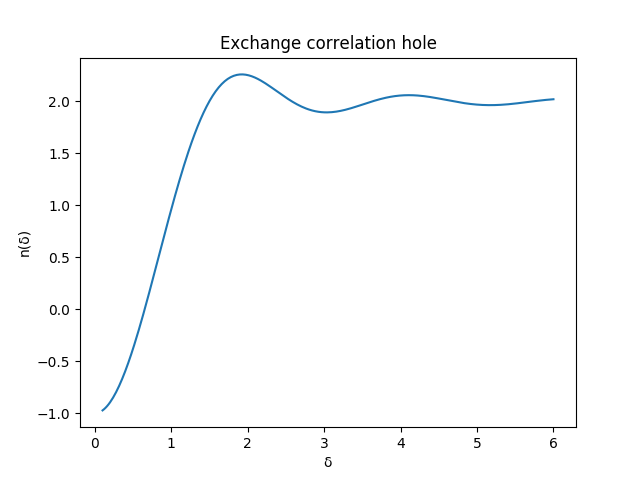
\includegraphics[width=130mm]{hole}
 \end{center}

 \captionof{figure}{Exchange correlation density}\label{fig:hole}\vspace{0.5cm}
 \end{solution}
\end{questions}

%
% \begin{center}
%   \includegraphics[width=55mm]{}
% \end{center}
%
% \captionof{figure}{}\label{new}\vspace{0.5cm}
